\documentclass[notitlepage]{article}
\usepackage{ctex}
\usepackage{amsmath}
\usepackage{amssymb}
\usepackage{indentfirst}
\usepackage{graphicx}
\usepackage{float}
\usepackage{subfig}
\usepackage{overpic}
\usepackage[a4paper, scale=0.85]{geometry}

\title{实验一\ 数据降维与分类任务}
\author{}
\date{}

\setlength{\parindent}{2em}
\linespread{2}

\begin{document}

\maketitle

\vspace{-7em}

\section{问题描述}

分别利用PCA和LDA降维技术对葡萄酒数据进行降维处理,在降维后的数据集上训练和测试logistic
回归分类器,并比较降维技术前后分类器准确率的变化。

\section{实现步骤与流程}

\subsection*{PCA降维}

求解样本的散布矩阵
\begin{equation*}
    \mathbf{S}(\boldsymbol{x}) = \sum_{i = 1}^{n} 
    (\boldsymbol{x}_{i} - \boldsymbol{\mu}_{x})
    (\boldsymbol{x}_{i} - \boldsymbol{\mu}_{x})^{\mathrm{T}}
\end{equation*}

求解散布矩阵最大的$\beta$个特征值对应的特征向量作为基向量进行投影
\begin{equation*}
    \mathbf{S}(\boldsymbol{x}) \boldsymbol{w}_{i} 
    = \lambda_{i} \boldsymbol{w}_{i}
    \qquad i = 1,\ 2,\ \cdots,\ k
\end{equation*}

投影后的样本特征向量
\begin{equation*}
    \boldsymbol{y} = \mathbf{W}^{\mathrm{T}} \boldsymbol{x} 
    \Rightarrow \mathbb{R}^{\beta} 
    = \mathbb{R}^{\beta \times \alpha} \mathbb{R}^{\alpha}
\end{equation*}

其中变换矩阵$\mathbf{W}$的列向量即为散布矩阵的特征向量$\boldsymbol{w}_{i}$

\subsection*{LDA降维}

求解类内散布矩阵
\begin{equation*}
    \mathbf{S}_{w}(\boldsymbol{x}) = \sum_{i = 1}^{c} \mathbf{S}_{i} = 
    \sum_{i = 1}^{c} \sum_{\boldsymbol{x} \in \mathcal{X}_{i}} 
    (\boldsymbol{x} - \boldsymbol{\mu}_{i})(\boldsymbol{x} - 
    \boldsymbol{\mu}_{i})^{\mathrm{T}}
\end{equation*}

求解类间散布矩阵
\begin{equation*}
    \mathbf{S}_{b}(\boldsymbol{x}) = \sum_{i = 1}^{c} n_{i} 
    (\boldsymbol{\mu}_{i} - \boldsymbol{\mu})
    (\boldsymbol{\mu}_{i} - \boldsymbol{\mu})^{\mathrm{T}}
\end{equation*}

如果类内散布矩阵可逆,投影的$\beta$个基向量满足
\begin{equation*}
    \mathbf{S}_{w}^{-1} \mathbf{S}_{b} \boldsymbol{w}_{i} 
    = \lambda_{i} \boldsymbol{w}_{i}
    \qquad i = 1,\ 2,\ \cdots,\ k
\end{equation*}

并且对应分别对应最大的$\beta$个特征值$\lambda_{i}$。如果类内散布矩阵不可逆,可以将其替换为
\begin{equation*}
    \mathbf{S}_{w} \leftarrow \mathbf{S}_{w} + 
    \epsilon \mathbf{I}_{\beta},\quad \epsilon > 0
\end{equation*}

投影后的样本特征向量
\begin{equation*}
    \boldsymbol{y} = \mathbf{W}^{\mathrm{T}} \boldsymbol{x} 
    \Rightarrow \mathbb{R}^{\beta} 
    = \mathbb{R}^{\beta \times \alpha} \mathbb{R}^{\alpha}
\end{equation*}

其中变换矩阵$\mathbf{W}$的列向量即为矩阵$\mathbf{S}_{w}^{-1} \mathbf{S}_{b}$
的特征向量$\boldsymbol{w}_{i}$

\subsection*{logistic回归}

logistic回归模型
\begin{equation*}
    \hat{y} = \sigma(z) = 
    \sigma(\boldsymbol{w}^{\mathrm{T}} \boldsymbol{x} + b)
\end{equation*}

其中$\sigma(\cdot)$代表sigmoid函数,对于logistic回归可以使用两种损失函数

\begin{itemize}
    \item 交叉熵损失
    \begin{equation*}
        \ell_{cross-entropy} = -\sum_{i = 1}^{n} \bigg[ y_{i} \log \hat{y}_{i} + 
        (1 - y_{i}) \log (1 - \hat{y}_{i}) \bigg]
    \end{equation*}
    \item 负对数似然
    \begin{equation*}
        \ell_{log-likelihood} = \sum_{i = 1}^{m} \left[-y_{i} \hat{y}_{i} +
        \log(1 + e^{\hat{y}_{i}}) \right]
    \end{equation*}
\end{itemize}

本次实验中采取前者进行实现。

\section{实验结果与分析}

由于实验要求的MindSpore框架相关的资料较为匮乏,因此本次实验采取开源机器学习算法库
sklearn与实验中的算法进行对比。sklearn是一个开源的基于python语言的机器学习工具包。
它通过numpy, scipy等python数值计算的库实现高效的算法应用,并且涵盖了几乎所有主流机器学习算法。

\subsection*{PCA降维}

经过实验算法以及sklearn算法的PCA降维后的样本如下图所示,可以看出,降维后的样本具有
较高的散布程度。并且样本经过实验的PCA算法降维后与sklearn的PCA算法相比拥有相同的性态,
但二者在某一特征维度上呈镜像对称。

\begin{figure*}[htbp]
	\centering
	\subfloat[PCA(实验)]{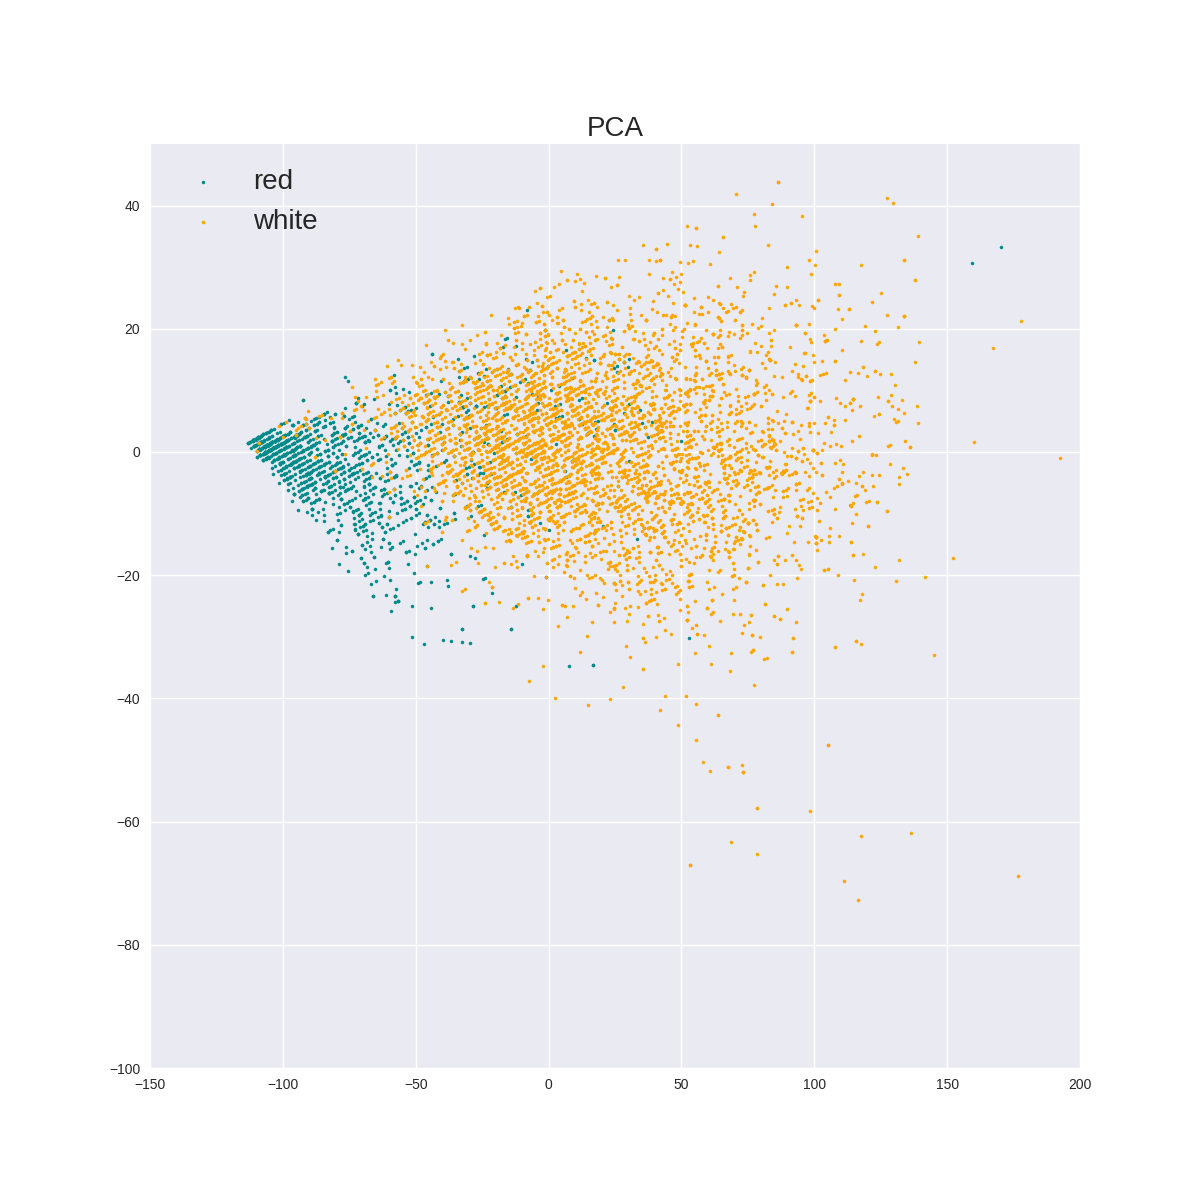
\includegraphics[width=.45\columnwidth]
    {../imgs/mine/pca_data.png}}\hspace{3pt}
	\subfloat[PCA(sklearn)]{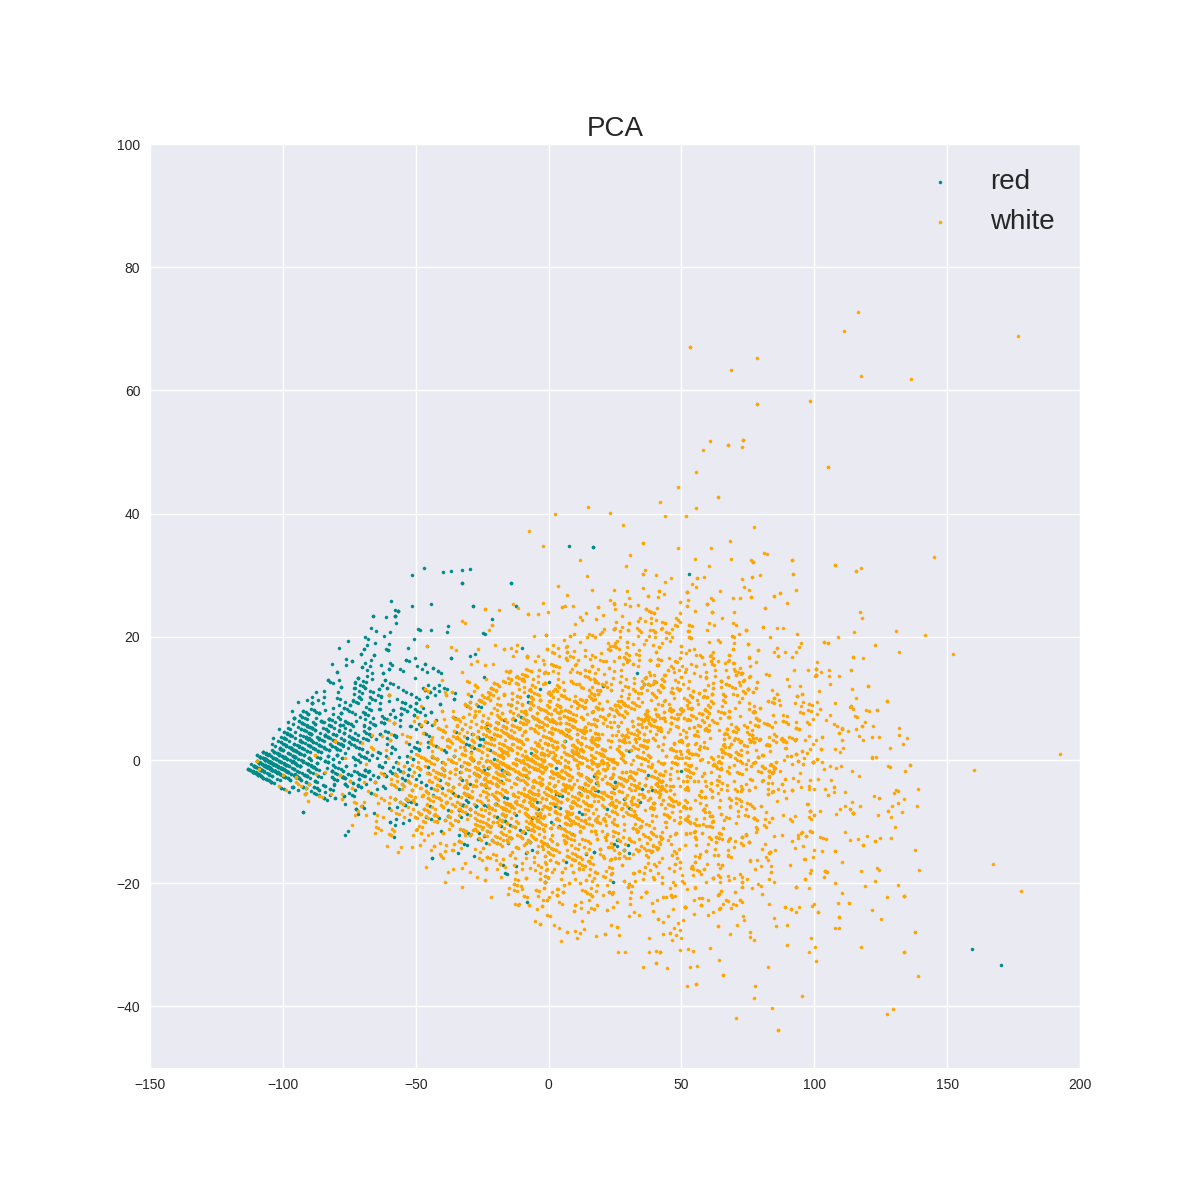
\includegraphics[width=.45\columnwidth]
    {../imgs/sklearn/pca_data.png}}
	\caption{PCA降维效果图}
\end{figure*}

\subsection*{LDA降维}

由于LDA限制降维维度不大于类别数减1,为了达到可视化的效果,本次实验仍然将样本降维到二维
经过实验算法降维后的样本如下图所示,可以看出,降维后的样本具有相对较好的可分性。
但无法展示sklearn的LDA降维效果图

\begin{figure*}[h]
	\centering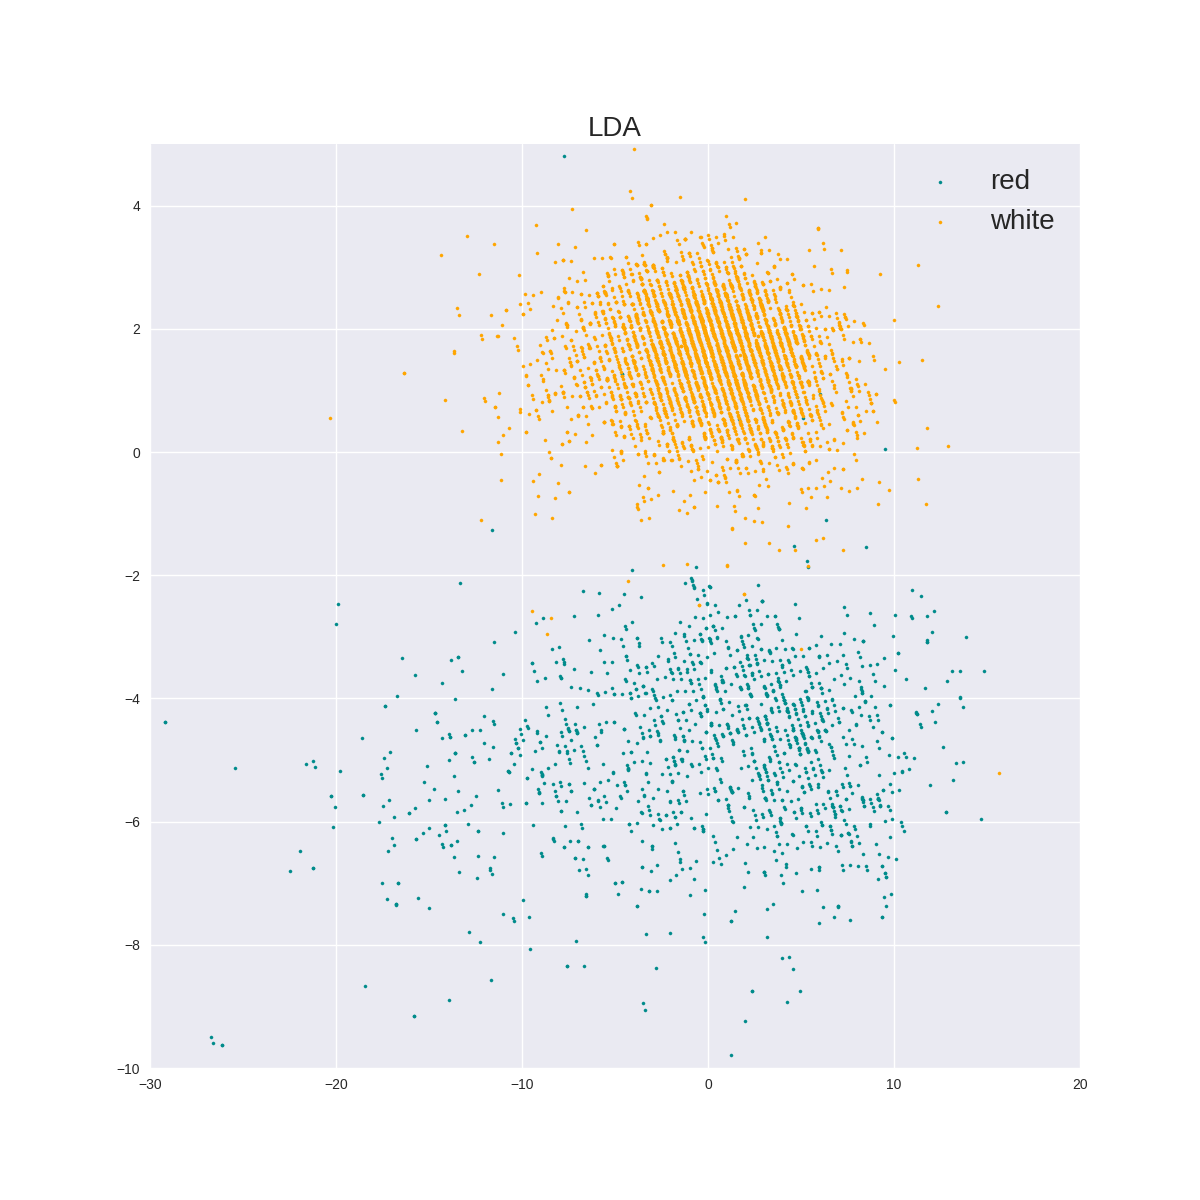
\includegraphics[width=.4\columnwidth]
    {../imgs/mine/lda_data.png}
	\caption{LDA降维效果图}
\end{figure*}

\subsection{logistic回归}

实验中实现的logistic回归在原始数据集、PCA降维数据集以及LDA降维数据集上的
训练过程如后图所示,分别展示了模型训练过程中损失函数以及分类准确率的变化。

\begin{figure*}[htbp]
	\centering
	\subfloat[训练历史(原始)]{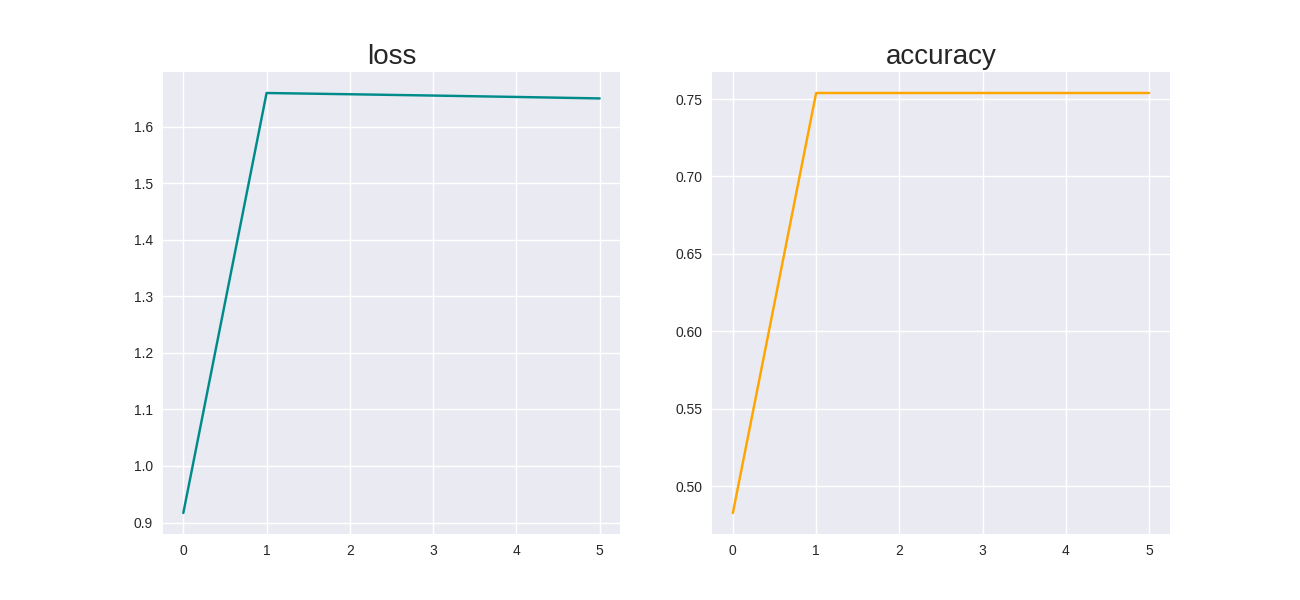
\includegraphics[width=.65\columnwidth]
    {../imgs/mine/origin_history.png}}\\
	\subfloat[训练历史(PCA)]{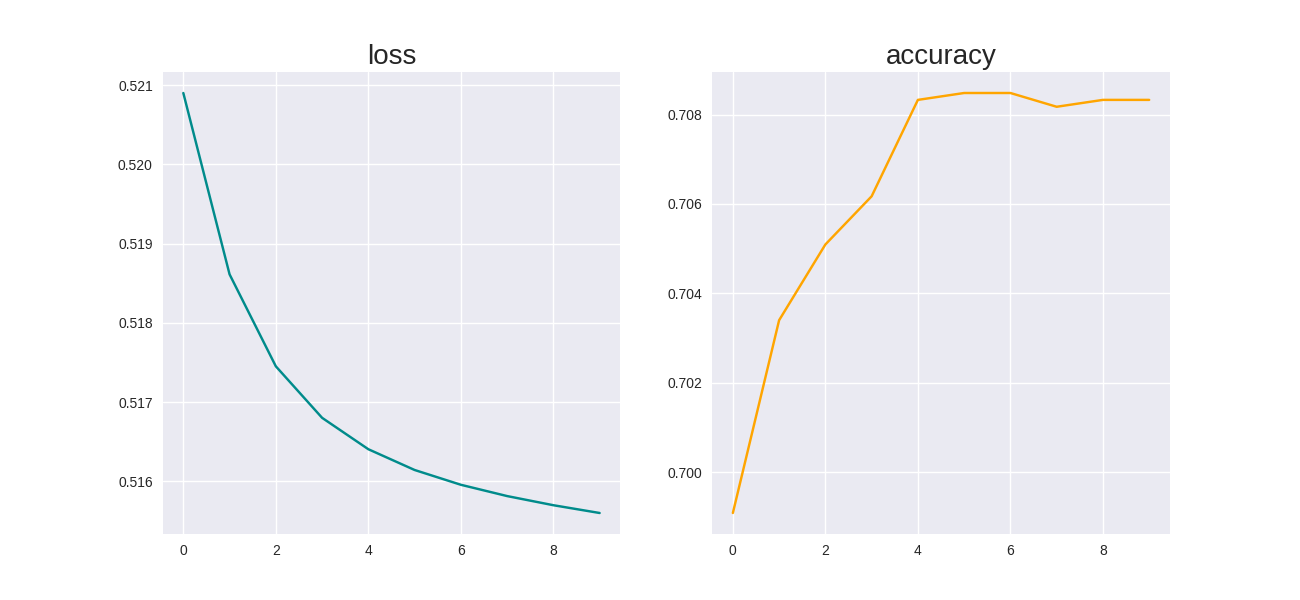
\includegraphics[width=.65\columnwidth]
    {../imgs/mine/pca_history.png}}\\
	\subfloat[训练历史(LDA)]{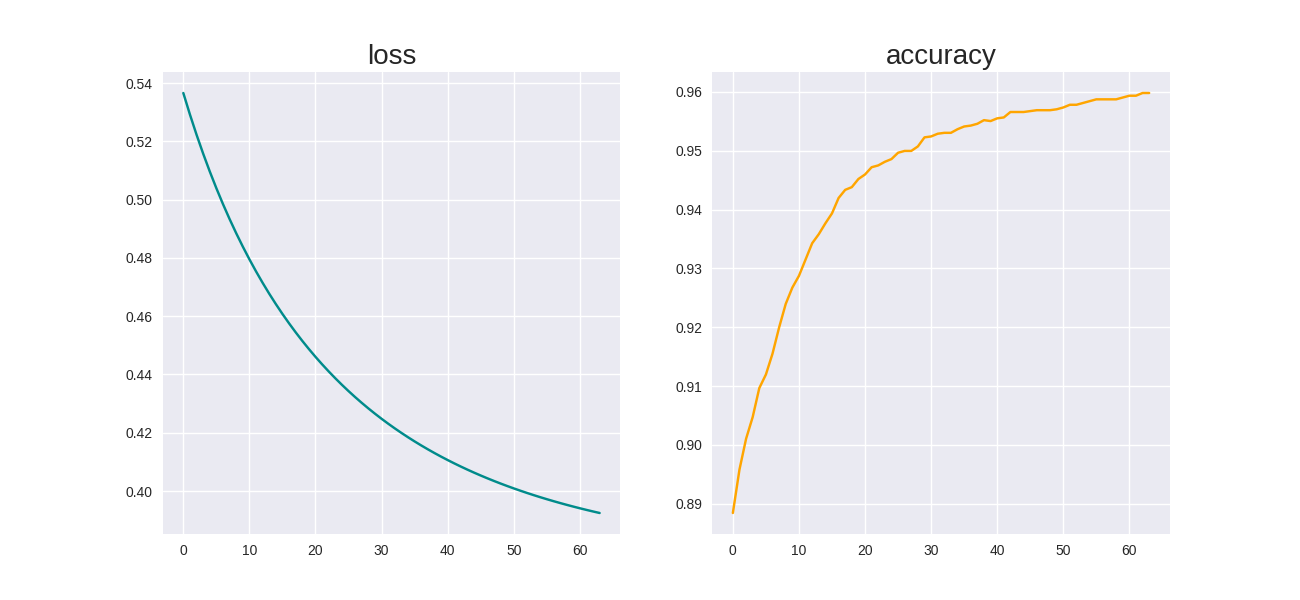
\includegraphics[width=.65\columnwidth]
    {../imgs/mine/lda_history.png}}
	\caption{logistic回归(实验)}
\end{figure*}

从图像中可以看出,原始数据集的模型准确率居中,PCA降维后的数据集的模型准确率较差,
LDA降维后的数据集的模型准确率最佳。

相应地,sklearn提供的logistic回归模型在各个数据集上的准确率如下图所示,与实验算法相同
的是,LDA的准确率最高,原始数据次之,PCA最低。
\begin{figure*}[htbp]
    \centering
    \includegraphics*[width=\columnwidth]{../imgs/sklearn/acc.png}
    \caption{logistic回归(sklearn)}
\end{figure*}

\section{MindSpore学习使用心得体会}

由于本次实验并未采用MindSpore,此部分用sklearn的学习使用心得体会来代替。

本次实验中调用了sklearn中的以下算法接口

\begin{itemize}
    \item PCA(decomposition PCA)
    \item LDA(discriminant\_analysis LinearDiscriminantAnalysis)
    \item logistic回归(linear\_model LogisticRegression)
\end{itemize}

作为实验算法的对照算法,sklearn提供的算法接口方便调用,并且执行效率较高,
能够高效地实现实验的需求。

\newpage

\section{代码附录}

\begin{figure*}[h]
    \centering
    \includegraphics*[width=\columnwidth]{../imgs/code.png}
    \caption{部分代码截图}
\end{figure*}

\end{document}